\chapter{Implementation of the Backend}

The focus of this chapter is on the implementation of the backend of the MiniC\verb|++| compiler. First, the differences between Java and C\verb|++| are presented. This is followed by the explanation of the source code generation. Finally, the generation of the bytecode is shown.

\section{Differences between Java and C\texttt{++}}

When compiling MiniC\verb|++| source code to Java bytecode, there are multiple differences in the functionality of both languages that need to be considered. The goal is to consider these differences and preserve the functionality of MiniC\verb|++| in bytecode. 

\subsection{Array Deletion}

MiniC\verb|++| includes the \verb|delete| keyword which reclaims the memory used for an array and invalidates the reference to it. Java on the other hand does not provide such a mechanism. In Java, the memory is managed by the JVM and the program can only request for the memory to be reclaimed by the garbage collector. To mimic MiniC\verb|++|'s behavior as best as possible, the delete statement is transformed into a null assignment (a = nullptr). Thus, if the array is only used inside one function, its memory can be reclaimed by the garbage collector. This solution however does not work if an array is passed as an input parameter into a function. This is because then a reference to the array will also exist in another function making it impossible to reclaim the memory.  

\subsection{cout and cin}

In MiniC\verb|++|, input and output to and from the console can be performed via the \verb|cout| and \verb|cin| streams. For output, Java uses the \verb|System.out| stream with separate methods for normal print and print with new line. All output statements therefore need to be transformed to either \verb|System.out.print| or \verb|System.out.println|. The latter one is used when an \verb|endl| is detected. 

For input, the \verb|java.util.Scanner| class can be used. The constructor of this class takes an input stream as a parameter. For the console in Java this is \verb|System.in|. The scanner then provides methods to conveniently read values of the types supported in MiniC\verb|++|, namely integer and boolean.

\subsection{Expression Evaluation}

MiniC\verb|++| allows for more complex expression evaluations than Java. An expression like $4 < 5 < 3$ is valid in MiniC\verb|++| but not in Java. The way this expression is evaluated is as follows: First the left side $4 < 5$ is evaluated resulting in either a 1 or a 0. Then this is compared to the 3, e.g., $0 < 3$, if the previous expression resulted in a 0. 

In Java this needs to be implemented as nested \verb|if| statements in the scheme of \verb|if (expr) ? 1 : 0|. If the expression is true then the result is a 1 and otherwise 0. The following expression then uses this result for its comparison.

\subsection{Function Declarations and Classes}

MiniC\verb|++| requires at least a declaration (or a full definition) of a function earlier in the source code file before it can be called. In Java however, methods can be used/called even if they are only defined later in the source code file. Therefore, there would be no need to enforce this rule, besides making sure that the function is actually defined at some point in the source code file. However, to honor this functionality of MiniC\verb|++|, a semantic exception is raised during the parse process if a reference of a function that is not yet declared is detected. 

MiniC\verb|++| does not include the concept of classes. Multiple functions are defined in a file but are not related to each other on a class level. In Java there can only be methods. Standalone functions outside of classes are not possible. To translate the MiniC\verb|++| source code to Java bytecode, all functions are put inside the same class. To mimic the behavior of MiniC\verb|++| as close as possible, all methods are defined as static methods.  

\section{Source Code Generation}

For the development of a compiler it is beneficial to implement a module for source code generation. The source code generation module takes the AST as input and generates MiniC\verb|++| source code. By generating source code from the AST, the correctness of the compiler frontend can be tested. If the code generated from the source code generator matches the original source code, it can be assumed that the AST has been correctly generated. When comparing there are some potential problems like formatting and comments. Therefore, it is best to take the generated source code and repeat the generation process one more time. The then generated source code can be used for comparison without any formatting or comments interfering. 

The implementation of the source code generator uses a StringBuilder combined with Kotlin extension functions. For each type of the AST, there is a \verb|generateSourceCode| extension function which takes a StringBuilder instance as the sole parameter. The extension functions are grouped according to their type into the following files:

\begin{itemize}
    \item \verb|BlockGenerator|,
    \item \verb|ConstVarDefGenerator|,
    \item \verb|ExprGenerator|,
    \item \verb|FuncGenerator|,
    \item \verb|MiniCppGenerator|,
    \item \verb|StatGenerator| and
    \item \verb|TypeGenerator|.
\end{itemize}

The code for the \verb|MiniCpp| AST node is shown in listing \ref{lst:SrcGenMiniCpp}. In this function, the String Builder is instantiated and eventually returned as a normal string. For each \verb|miniCppEntry| the respective \verb|generateSourceCode| function is called. The code to generate the \verb|ConstDef| node is shown in listing \ref{lst:SrcGenConstDef}. First, the \verb|const| keyword is added to the String Builder, followed by the source code for the type. Then all identifiers with their respective values are appended to the String Builder. On the last entry, the delimiter is omitted. 


\begin{KotlinCode}[float,numbers=none,caption=Implementation of the \texttt{generateSourceCode} method for the \texttt{MiniCpp} class., label=lst:SrcGenMiniCpp]
fun MiniCpp.generateSourceCode(): String {
    val sb = StringBuilder()
    entries.forEach {
        when (it) {
            is ConstDef -> it.generateSourceCode(sb)
            is FuncDecl -> it.generateSourceCode(sb)
            is FuncDef  -> it.generateSourceCode(sb)
            Sem         -> sb.appendLine(";")
            is VarDef   -> it.generateSourceCode(sb)
        }
    }
    return sb.toString()
}
\end{KotlinCode}
    

\begin{KotlinCode}[float,numbers=none,caption=Implementation of the \texttt{generateSourceCode} method for the \texttt{ConstDef} class., label=lst:SrcGenConstDef]
fun ConstDef.generateSourceCode(sb: StringBuilder) {
    sb.append("const ")
    type.generateSourceCode(sb)
    sb.append(" ")
    entries.forEachIndexed { index, entry ->
        sb.append("${entry.ident.name} = ")
        entry.value.generateSourceCode(sb)
        if (index != entries.lastIndex) {
            sb.append(", ")
        }
    }
    sb.appendLine(";")
}
\end{KotlinCode}

\section{Classes}

The first step when generating bytecode is to handle everything that is relevant on a class level. Every piece of code in Java is organized inside a class and stored inside a \verb|.class| file. For this task, the ASM framework provides the \verb|ClassWriter| class. This class provides visitor pattern based methods for generating a class file. The code for generating the class definition is shown in listing \ref{lst:BtGenClassDef}. The constructor for the \verb|ClassWriter| takes an integer parameter that functions as a flag which modifies the behavior of the class writer. In this case, the \verb|COMPUTE_FRAMES| and  \verb|COMPUTE_MAXS| flags are used. \verb|COMPUTE_FRAMES| enables the computation of stack map frames of methods from the bytecode. Further, \verb|COMPUTE_MAXS| calculates the maximum stack size from the bytecode. Those two flags combined ease the development of the code generation since those two aspects are now computed automatically. Otherwise, it would be necessary to keep track of those values manually for every method generation, increasing complexity. 

The \verb|visit| method defines a class. The first parameter is the \verb|CLASS_FILE_VERSION| constant which has the value 65. This corresponds to Java version 21. The second parameter defines the access flags of the class. \verb|ACC_PUBLIC| means that the class is public. The third parameter is the class name. The fourth parameter defines the signature of the class, which is only relevant for generic classes and therefore left as \verb|null|. The superclass is described by the fifth parameter. As the concept of classes does not exist in MiniC\verb|++| Java's default superclass \verb|java.lang.Object| is used as the superclass. Via the last parameter, implemented interfaces can be defined. This parameter is also set to \verb|null| as MiniC\verb|++| does not support interfaces.

\begin{KotlinCode}[float,numbers=none,caption=Code for the definition of a class., label=lst:BtGenClassDef]
val classWriter = ClassWriter(ClassWriter.COMPUTE_FRAMES + ClassWriter.COMPUTE_MAXS)
className = miniCpp.className
classWriter.visit(
    CLASS_FILE_VERSION,
    ACC_PUBLIC,
    miniCpp.className,
    null,
    "java/lang/Object",
    null
)
\end{KotlinCode}


Once the class has been initialized, the bytecode generation based on the AST can begin. On the top level, this process is shown in listing \ref{lst:BtGenTopLevelCode}. First, a \verb|StaticVarDefGenerator| is instantiated. The same instance is used across the entire generation process, since the generation of static variable definitions requires the modification of the static class initializer block. Then, for each \verb|miniCppEntry| the appropriate bytecode is generated. For \verb|Sem| and \verb|FuncDecl| no code needs to be generated, since they don't encode any semantic information relevant for bytecode. The \verb|addStaticScannerField| adds a scanner to the static variables. This is needed for the generation of \verb|cin| statements. To make the class executable, a main method is needed. This is done via the \verb|addMainMethod| method. Calling the \verb|visitEnd| method of the \verb|classWriter| finishes the code generation for the class. Finally, calling the \verb|toByteArray| method returns the bytecode of the generated class as a byte array. 

\begin{KotlinCode}[float,numbers=none,caption=Top-level code for the bytecode generation., label=lst:BtGenTopLevelCode]
val staticVarDefGenerator = StaticVarDefGenerator(classWriter)
miniCpp.entries.forEach {
    when (it) {
       is VarDef   -> staticVarDefGenerator.generateStatic(it)
       is ConstDef -> StaticConstDefGenerator(classWriter).generateStatic(it)
       is FuncDef  -> FuncDefGenerator(classWriter, miniCpp.className).generate(it)
       is Sem,
       is FuncDecl -> ""
    }
}
staticVarDefGenerator.generateStaticInitBlock(miniCpp)
addStaticScannerField(classWriter)
addMainMethod(classWriter)
classWriter.visitEnd()
return classWriter.toByteArray()
\end{KotlinCode}

\section{Functions}

A function in MiniC\verb|++| is translated into a class method in bytecode. The \verb|FuncGenerator| accepts a \verb|FuncDef| AST node and generates the bytecode for it. The code for the generation is shown in listing \ref{lst:BtGenFuncGen}. To generate code for a method a \verb|MethodVisitor| instance is needed. The visitor can be acquired by calling the \verb|visitMethod| method of the class writer. The parameter of the \verb|visitMethod| defines the signature of the method to be generated. The first parameter defines the access of the method. \verb|ACC_PUBLIC| and \verb|ACC_STATIC| define that the method has the modifiers \verb|public| and \verb|static|. The second parameter is the name of the method. The third parameter defines the method's descriptor. The descriptor is a string representation of the input parameter types and the return type of the method. The fourth parameter describes the method's signature. This parameter is only needed for generics and thus can be set to \verb|null|. The final parameter is a string array containing all exceptions that the method may throw. Since  it is not possible in MiniC\verb|++| to write code that would cause a checked exception, this parameter can also be set to \verb|null|. 

\begin{KotlinCode}[float,numbers=none,caption=Code for the bytecode generation of the \texttt{FuncDef} node., label=lst:BtGenFuncGen]
fun generate(funcDef: FuncDef) {
    val methodVisitor = classWriter.visitMethod(
        Opcodes.ACC_PUBLIC + Opcodes.ACC_STATIC,
        funcDef.funHead.ident.name,
        funcDef.funHead.getDescriptor(),
        null,
        null
    )
    methodVisitor.run {
        visitCode()
        BlockGenerator(methodVisitor, className).generate(funcDef.block, null)
        visitInsn(RETURN)
        visitMaxs(0, 0)
        visitEnd()
    }
}
\end{KotlinCode}


Listing \ref{lst:BtGenFuncGenDesc} shows the generation of the descriptor. The descriptor is generated using a String Builder. The input parameter types are grouped inside parenthesis. \verb|void| or empty input parameters are represented as \verb|()|. For each input parameter it's type descriptor is added to the method descriptor. The following descriptors are relevant for the code generation from MiniC\verb|++|:

\begin{itemize}
    \item Void:           \verb|V|,
    \item Boolean:        \verb|Z|,
    \item Integer:        \verb|I|,
    \item Boolean Array: \verb|[Z| and
    \item Integer Array: \verb|[I|.
\end{itemize}

Once the input parameters are added, the descriptor of the return type is appended after the closing parenthesis. E.g., For a method with an integer and boolean input parameter and a boolean return type the descriptor is \verb|(IZ)Z|.


\begin{KotlinCode}[float,numbers=none,caption=Generation of the descriptor of a method., label=lst:BtGenFuncGenDesc]
fun FuncHead.getDescriptor(): String {
    val descriptor = StringBuilder("(")
    if (formParList != null && formParList is FormParListEntries) {
        (formParList as FormParListEntries).entries.forEach {
            descriptor.append(it.type.descriptor)
        }
    }
    descriptor.append(")")
    descriptor.append(type.descriptor)
    return descriptor.toString()
}
\end{KotlinCode}

Listing \ref{lst:BtGenFuncGen} further shows the code generation for the method's body. The \verb|run| extension function changes the \verb|this| of the functions body to the \verb|methodVisitor|. With this, the methods of it can be called without having to explicitly type \verb|methodVisitor|. To start the code generation the \verb|visitCode| method is called. All following visitor calls are then added to the method's body. The method's body is generated by the \verb|BlockGenerator|. The \verb|BlockGenerator| calls the respective code generators for each \verb|blockEntry|. Namely, the \verb|LocalVarDefGenerator| and the \verb|StatGenerator|. For constant definitions, no code needs to be generated at the definition stage. Since every method needs a return instruction, even if the method's return type is \verb|void|, a return instruction is added after the \verb|BlockGenerator|. For normal instructions like \verb|RETURN|, the \verb|visitInsn| method is used. The \verb|visitMaxs| method call sets the maximum stack size and maximum size of the local variables. Both are set to zero as the ASM framework computes the correct values based on the generated bytecode. To finish the code generation for the method the \verb|visidEnd| method is called.  

\section{Static Fields}

Variable definitions of MiniC\verb|++| are converted to static variables inside the class. Constant definitions are added to the constant pool. When a constant variable is referenced inside the bytecode, the value from the constant pool is loaded. 

\subsection{Constant Definitions}

Constant definitions are handled by the \verb|StaticConstDefGenerator| class. Its source code is visible in listing \ref{lst:BtGenConstDefGen}. The generator takes the \verb|ClassWriter| instance as a constructor argument, so that the constant pool can be accessed. In the \verb|generateStatic| method, a \verb|ConstDef| node is accepted and processed. ASM provides the \verb|newConst| method that creates an entry in the constant pool of the class and returns the index of the value in it. If an entry with the same value already exists, its index is returned instead. For all \verb|constDefEntry| elements this method is called, and the index is stored in the variable associated with it. When the constant is referenced later, the index can be used to put the value on the operand stack.


\begin{KotlinCode}[float,numbers=none,caption=Code of the \texttt{StaticConstDefGenerator} class., label=lst:BtGenConstDefGen]
class StaticConstDefGenerator(private val cw: ClassWriter) {

    fun generateStatic(constDef: ConstDef) {
        constDef.entries.forEach { entry ->
            val index = cw.newConst(entry.value.value.getValue())
            entry.variable.index = index
        }
    }
}
\end{KotlinCode}

\subsection{Variable Definitions}

The \verb|StaticVarDefGenerator| class generates the code for static variable definitions. In bytecode, the declaration and initialization are split up. First, the field is defined and then later in the static initializer block of the class, a value is assigned to it.

Listing \ref{lst:BtGenStatVarDecl} shows the code for the declaration of a static variable. The \verb|ClassWriter| method \verb|visitField| declares the variable. The first parameter defines the access flags, in this case all variables are \verb|public| and \verb|static|. The second parameter defines the name of the variable. Contrary to local variables which use indexes, static variables are referenced by their name. The type of the variable is defined by the third parameter. For this, the type descriptor is used. The fourth parameter handles the variable's signature. It can be set to \verb|null|, because no generics are used. The final parameter sets the value of the field. This field is only relevant for \verb|final| variables, whose value cannot change. Each \verb|VarDef| node is also added to the \verb|generatedVarDefs| list, which is used for the initialization.



\begin{KotlinCode}[float,numbers=none,caption=Code for the declaration of static variables., label=lst:BtGenStatVarDecl]
fun generateStatic(varDef: VarDef) {
    varDef.entries.forEach { entry ->
        cw.visitField(
            ACC_PUBLIC
                    or ACC_STATIC,
            entry.ident.name,
            varDef.type.toPointerTypeOptional(entry.pointer).descriptor,
            null,
            null
        )
    }
    generatedVarDefs.add(varDef)
}
\end{KotlinCode}

The initialization is performed by the code shown in listing \ref{lst:BtGenStatVarInit}. First, the method visitor for the static initializer block is acquired by calling the \verb|visitMethod| method. The name of the static initializer block is predefined with \verb|<clinit>| and the method has no parameters and the \verb|void| return type. For all \verb|VarDef| entries with no default, values are filtered. For each entry its default value is pushed onto the operand stack as a constant using the \verb|visitLdcInsn| method. The \verb|visitFieldInsn| method then pops the value from the operand stack and assigns it to the static variable. The first parameter of the method is the operand code. \verb|PUTSTATIC| is the operand code for assigning a new value to a static variable. The second parameter describes the owner of the variable, in this case it is the current class name. The third parameter is the identifier and the final one the descriptor of the variable type.

The \verb|visitScannerInit| method initializes the scanner which is used to read input from the console. First, the method ensures that the name for the scanner variable is not taken by looking through all scopes. Then, an instance of the scanner is initialized. To invoke the constructor the op code \verb|INVOKESPECIAL| is used.

%potentially code for scanner

\begin{KotlinCode}[float,numbers=none,caption=Code for the initialization of static variables., label=lst:BtGenStatVarInit]
fun generateStaticInitBlock(miniCpp: MiniCpp) {
    cw.visitMethod(
        ACC_STATIC,
        "<clinit>",
        "()V",
        null,
        null
    ).apply {
        visitCode()
        generatedVarDefs.forEach { varDef ->
            varDef.entries
                .filter{ it.value != null }
                .forEach { entry ->
                visitLdcInsn(entry.value?.value?.getValue())
                visitFieldInsn(
                    PUTSTATIC,
                    miniCpp.className,
                    entry.ident.name,
                    varDef.type.toPointerTypeOptional(entry.pointer).descriptor
                )
            }
        }
        visitScannerInit(miniCpp)
        visitInsn(RETURN)
        visitMaxs(0, 0)
        visitEnd()
    }
}
\end{KotlinCode}

\section{Local Variables}

MiniC\verb|++| supports local variables and constant definitions. The latter one are handled in the same way as the global constant definitions by the \verb|ConstDefGenerator|. For each constant definition, an entry is created in the constant pool of the class. When the constant definition is referenced, the constant's value is pushed onto the operand stack from the constant pool.

The \verb|LocalVarDefGenerator| generates the code for local variable definitions. The relevant bytecode is generated by the code shown in listing \ref{lst:BtGenVarDef}. First, for each entry the type is optionally converted to a pointer type, if the flag is set. Then the \verb|pushInitValue| method takes the entry's value and pushes it onto the stack. In case the value is null, the respective default value of the type is pushed onto the stack. The \verb|storeVariable| method then stores the value from the stack in the variable. For this, the variable type and index is needed. Depending on the type of the variable, a different opcode needs to be generated. The bytecode instruction is generated by the \verb|visitVarInsn| method, which takes the opcode and the index of the variable as a parameter. 


\begin{KotlinCode}[float,numbers=none,caption=Code for the definition of local variables., label=lst:BtGenVarDef]
fun generate(varDef: VarDef) {
    varDef.entries.forEach { entry ->
        val type = varDef.type.toPointerTypeOptional(entry.pointer)
        pushInitValue(entry.value, type)
        storeVariable(type, entry.variable.index)
    }
}

private fun storeVariable(type: ExprType, index: Int) {
    val opCode = when (type) {
        ExprType.INT  -> ISTORE
        ExprType.BOOL -> ISTORE
        else          -> ASTORE
    }
    mv.visitVarInsn(opCode, index)
}
\end{KotlinCode}

\section{Statments}

Statements are generated by the \verb|StatGenerator| class. When generating a statement, first the appropriate generation method for the specific type of statement is chosen. This is done by the \verb|generate| method of the \verb|StatGenerator| shown in listing \ref{lst:BtGenStatGen}. Depending on the complexity of the statement, the code is generated by another generator, e.g., the \verb|OutputStatGenerator|. The \verb|BreakStat| requires just one instruction and is thus generated directly in the method. The \verb|EmptyStat| does not lead to the generation of any bytecode and is ignored. 

\begin{KotlinCode}[float,numbers=none,caption=Implementation of the \texttt{generate} method of the \texttt{StatGenerator}., label=lst:BtGenStatGen]
fun generate(stat: Stat, breakLabel: Label?) {
    when (stat) {
        is InputStat -> generateInputStat(stat)
        is BlockStat -> BlockGenerator(mv, className).generate(stat.block, breakLabel)
        is DeleteStat -> generateDeleteStat(stat)
        is ReturnStat -> generateReturnStat(stat)
        is OutputStat -> OutputStatGenerator(mv).generate(stat)
        is ExprStat -> ExprGenerator(mv).generate(stat.expr, false)
        is WhileStat -> generateWhileStat(stat)
        is IfStat -> generateIfStat(stat, breakLabel)
        is BreakStat -> mv.visitJumpInsn(Opcodes.GOTO, breakLabel!!)
        is EmptyStat -> ""
    }
}
\end{KotlinCode}

\subsection{If Statement}

The transformation of an if statement to bytecode is visualized in figure \ref{fig:IfStat}. An if statement is generated by the \verb|generateIfStat| method shown in listing \ref{lst:BtGenIfStatGen}. First, two labels are created. Bytecode uses labels as the target for its \verb|GOTO| instructions. For if statements, two labels are needed, one for the else branch and one to mark the end of the statement. Then the bytecode for the if statement's condition is generated by the \verb|ExprGenerator|. The jump instruction \verb|IFEQ| then checks if the top value on the stack is equal to zero. If this is the case, a jump to the \verb|elseLabel| is performed. Otherwise, the execution proceeds to the next instruction. The code for the \verb|thenStat| is generated by the \verb|generate| method of the \verb|StatGenerator|. After that, a jump to the end of the statement is generated. This is done, because the else branch of the if statement is generated after the then branch and thus needs to be skipped. If an else branch is present, the bytecode for it is generated in the same way.


\begin{figure}[]
    \centering
    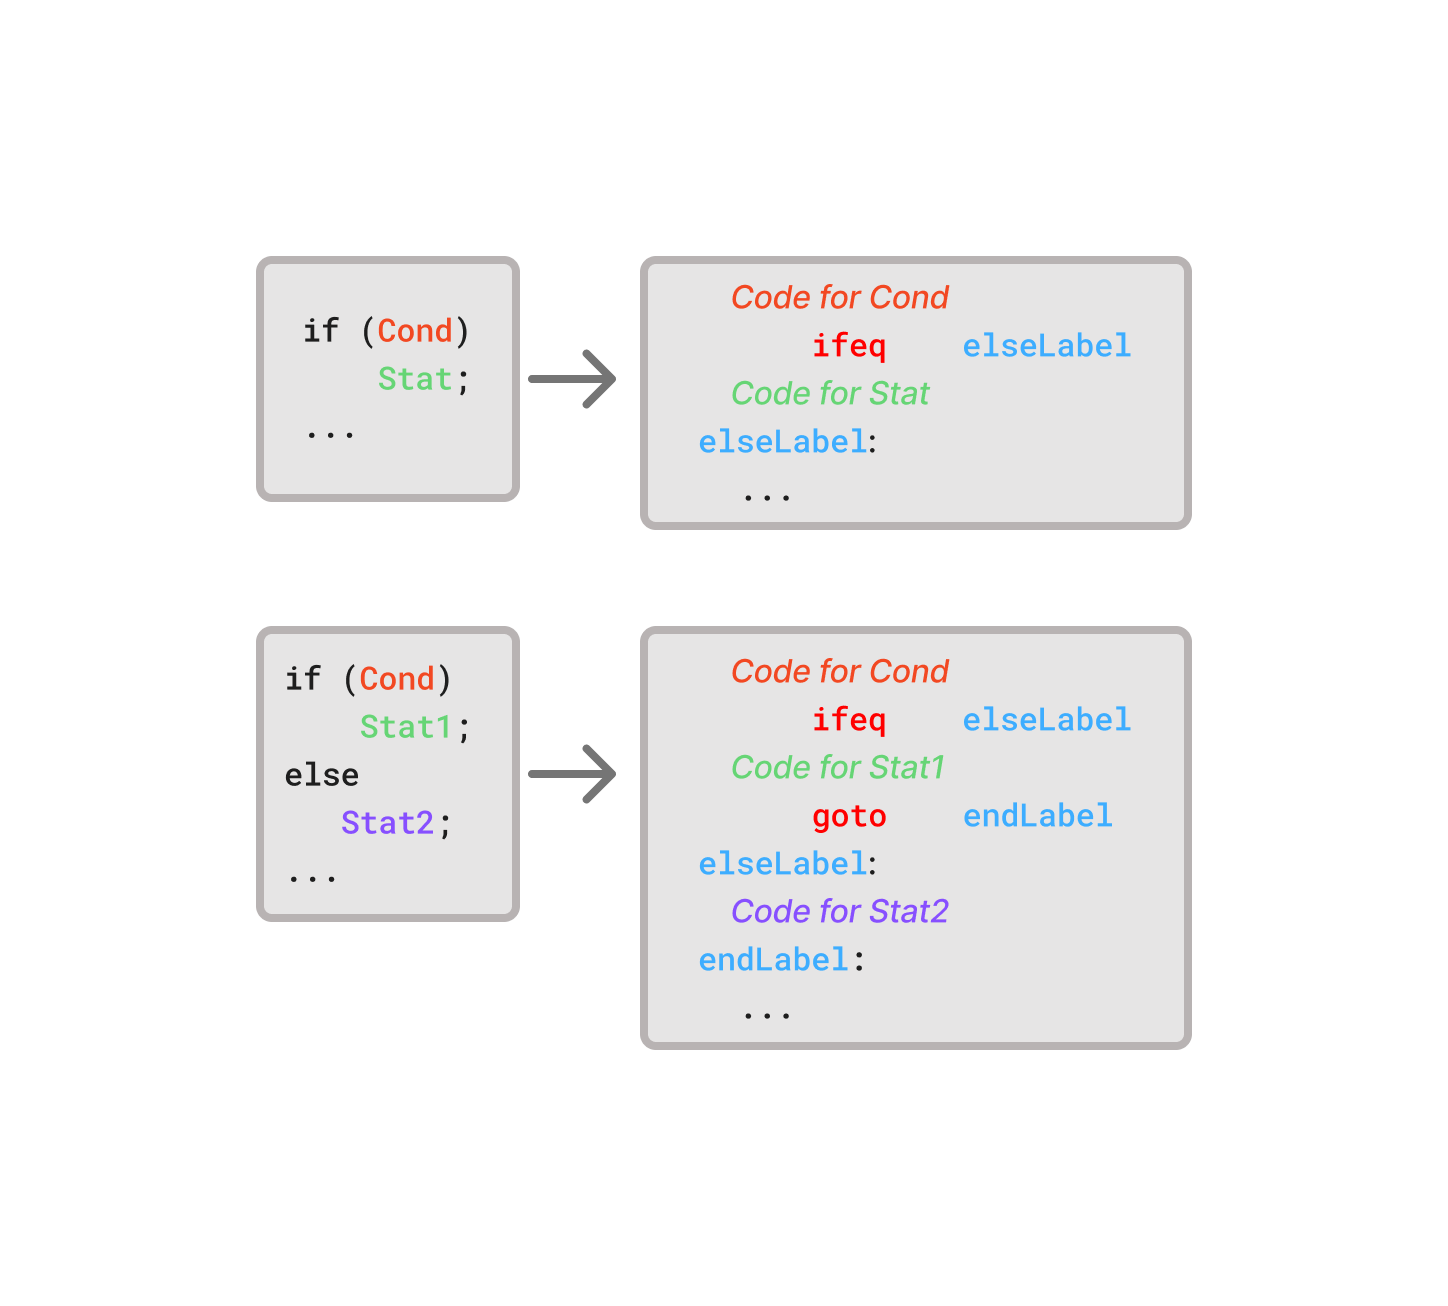
\includegraphics[width=\textwidth]{ifstat.png}
    \caption{Transformation of an if statement to bytecode.}
    \label{fig:IfStat}
\end{figure}


\begin{KotlinCode}[float,numbers=none,caption=Implementation of the \texttt{generateIfStat} method of the \texttt{StatGenerator}., label=lst:BtGenIfStatGen]
private fun generateIfStat(stat: IfStat, breakLabel: Label?) {
    val elseLabel = Label()
    val endLabel = Label()

    ExprGenerator(mv).generate(stat.condition)
    mv.visitJumpInsn(Opcodes.IFEQ, elseLabel)
    generate(stat.thenStat, breakLabel)
    mv.visitJumpInsn(Opcodes.GOTO, endLabel)
    mv.visitLabel(elseLabel)
    stat.elseStat?.let { generate(it, breakLabel) }
    mv.visitLabel(endLabel)
}
\end{KotlinCode}

\subsection{Delete Statement}

The delete statement causes the reference to the array to be set to null. Reclaiming memory in the same way as in \verb|C++| is not possible in the JVM. The bytecode generation for the delete statement is shown in figure \ref{lst:BtGenDeleteStatGen}. First, the variable associated with the identifier specified in the delete statement is retrieved. The \verb|ACONST_NULL| opcode pushes a \verb|null| value onto the stack. With the \verb|ASTORE| opcode the value is then popped from the stack and assigned to the array variable. 


\begin{KotlinCode}[float,numbers=none,caption=Implementation of the \texttt{generateDeleteStat} method of the \texttt{StatGenerator}., label=lst:BtGenDeleteStatGen]
private fun generateDeleteStat(stat: DeleteStat) {
    val variable = stat.scope.getVariable(stat.ident)
    mv.visitInsn(Opcodes.ACONST_NULL)
    mv.visitVarInsn(Opcodes.ASTORE, variable.index)
}
\end{KotlinCode}

\subsection{Input Statement}

The input statement reads a value from the console and then assigns that value to a variable. To read a value from the console, the static \verb|Scanner| instance is used. The code implementing the input statement is shown in listing \ref{lst:BtGenInputStatGen}. The scanner is loaded with the \verb|GETSTATIC| opcode, and it's owner, name and descriptor. The method of the scanner, that should be called, depends on the type of the variable. To invoke a method of an object, the \verb|INVOKEVIRTUAL| opcode is needed. The method visitor generates method invocations using the \verb|visitMethodInsn| method. In addition to the opcode, the qualified name of the scanner, method name, descriptor and a boolean value indicating if the method comes from a class or interface. Finally, the value put onto the stack by the scanner is stored. In case the variable is static, the \verb|visitFieldInsn| method is used to store the value with the \verb|PUTSTATIC| opcode. The \verb|visitVarInsn| method in combination with the \verb|ISTORE| opcode, stores the value for a local variable. 


\begin{KotlinCode}[float,numbers=none,caption=Implementation of the \texttt{generateInputStat} method of the \texttt{StatGenerator}., label=lst:BtGenInputStatGen]
private fun generateInputStat(stat: InputStat) {
    mv.visitFieldInsn(GETSTATIC, className, scannerVarName, SCANNER_DESC)
    val variable = stat.scope.getVariable(stat.ident)
    val methodName = if (variable.type == ExprType.INT) "nextInt" else "nextBoolean"
    val methodDesc = if (variable.type == ExprType.INT) "()I" else "()Z"
    mv.visitMethodInsn(
        Opcodes.INVOKEVIRTUAL,
        SCANNER_QUAL_NAME,
        methodName,
        methodDesc,
        false
    )
    if(variable.static) {
        mv.visitFieldInsn(
            Opcodes.PUTSTATIC,
            className,
            variable.ident.name,
            variable.type.descriptor
        )
    } else {
        mv.visitVarInsn(Opcodes.ISTORE, variable.index)
    }
}
\end{KotlinCode}

\subsection{While Statement}

The transformation of a while statment to bytecode is shown in figure \ref{fig:WhileStat}. Listing \ref{lst:BtGenWhileStatGen} shows the code for the generation of a while statement. A while statement requires two labels. One for the start and one for the end of the statement. The start label is marked with the \verb|visitLabel| method of the method visitor. Then, the condition's bytecode is generated by the \verb|ExprGenerator|. The condition is then checked with the \verb|IFEQ| opcode that jumps to the specified label in the case the condition matches the value zero. If the condition is true, the body of the while statement is executed. It is generated by the \verb|generate| method of the \verb|StatGenerator|. The \verb|endLabel| is passed as a parameter. In the case that somewhere in the statement's body a \verb|break| statement is defined, it will jump to this label. At the end of the statement's body the loop is repeated by jumping to the \verb|startLabel| with the \verb|GOTO| opcode. The \verb|endLabel| is visited after the jump instruction. 

\begin{figure}[]
    \centering
    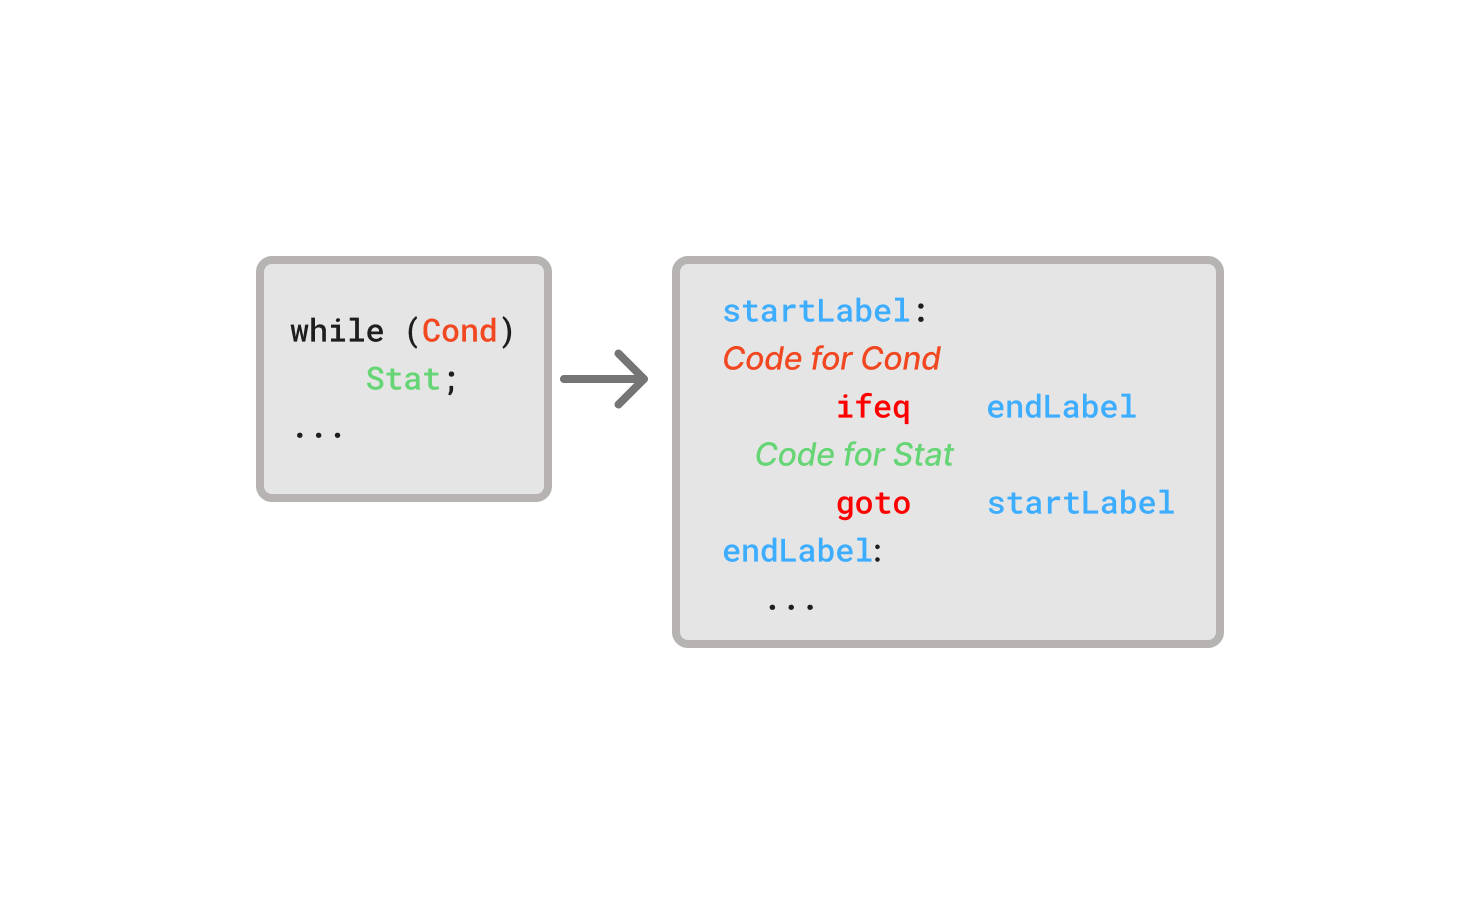
\includegraphics[width=\textwidth]{whileStat.png}
    \caption{Transformation of a while statement to bytecode.}
    \label{fig:WhileStat}
\end{figure}

\begin{KotlinCode}[float,numbers=none,caption=Implementation of the \texttt{generateInputStat} method of the \texttt{StatGenerator}., label=lst:BtGenWhileStatGen]
private fun generateWhileStat(stat: WhileStat) {
    val startLabel = Label()
    val endLabel = Label()
    mv.visitLabel(startLabel)
    ExprGenerator(mv).generate(stat.condition)
    mv.visitJumpInsn(Opcodes.IFEQ, endLabel)
    generate(stat.whileStat, endLabel)
    mv.visitJumpInsn(Opcodes.GOTO, startLabel)
    mv.visitLabel(endLabel)
}
    \end{KotlinCode}

\subsection{Output Statement}

Output statements are handled by the \verb|OutputStatGenerator| which generates the bytecode for \verb|System.out.print| and \verb|System.out.println| calls. An output statement consists of one or more \verb|outputStatEntry| elements, which can be expressions, string literals or end of line token. Before the code generation for each type, the \verb|System.out| static field is loaded. For an expression, it's bytecode is generated by the \verb|ExprGenerator|. The descriptor for the \verb|print| method is selected based on the type of the expression. The descriptor is then passed on to the \verb|generatePrint| method, which generated bytecode for the \verb|print| method invocation. The qualified name of the \verb|out| print stream is \texttt{java/io/PrintStream}. To print a stream literal, its value is put onto the stack using the \verb|visitLdcInsn| method. To print a string, the \verb|generatePrint| method must be passed the descriptor of the \verb|String| type, which is \texttt{(Ljava/lang/String;)V}. 


\begin{KotlinCode}[float,numbers=none,caption=Code for the print generation methods of the \texttt{OutputStatGenerator}., label=lst:BtGenOutputStatGen]
private fun generatePrintExpr(expr: Expr) {
    ExprGenerator(mv).generate(expr)
    val descriptor = if (expr.getType() == ExprType.INT) {
        PRINT_INT_DESC
    }else {
        PRINT_BOOL_DESC
    }
    generatePrint(descriptor)
}

private fun generatePrintText(text: String) {
    mv.visitLdcInsn(text)
    generatePrint(PRINT_STRING_DESC)
}

private fun generatePrint(descriptor: String) {
    mv.visitMethodInsn(
        INVOKEVIRTUAL,
        PRINT_STREAM_QUALIFIED_NAME,
        PRINT_METHOD_NAME,
        descriptor,
        false
    )
}
\end{KotlinCode}


\section{Expressions}

The \verb|ExpressionGenerator| is the root class for the bytecode generation of expressions. Each child type of \verb|Expr| has its own generator class. The generation process begins in the \verb|generate| method of the \verb|ExpressionGenerator| shown in listing \ref{lst:BtGenExprGenGen}. If the \verb|exprEntries| list is empty then the code generation is delegated to the \verb|OrExprGenerator|. Otherwise, the expression performs an assignment. 

The \verb|mapToAssignPairs| extension function maps the \verb|OrExpr| in the \verb|exprEntry| to the assignment operator that is used on it and returns a list of all such pairs. The last pair (the most right assignment), does not include an assignment operator. The values of all entries are then put onto the stack by the \verb|putExprValuesOnStack| extension function shown in listing \ref{lst:BtGenExprGenValStack}. This process is performed for all assignment types except the standard assign (\verb|=|). The values need to be put on the stack to have them ready for the calculation that needs to be performed for an assignment like \verb|+=| or \verb|%=|. 


% = generation only on most right one cus duplicate to left

\begin{KotlinCode}[float,numbers=none,caption=Implementation of the \texttt{generate} method of the \texttt{ExpressionGenerator}., label=lst:BtGenExprGenGen]
fun generate(expr: Expr, shouldEmitValue: Boolean = true) {
    val generator = OrExprGenerator(mv)
    if (expr.exprEntries.isEmpty()) {
        generator.generate(expr.firstExpr, shouldEmitValue)
    } else {
        val exprEntries = expr.mapToAssignPairs()
        generator.putExprValuesOnStack(exprEntries)
        generator.generateAssignCode(exprEntries)
    }
}  
\end{KotlinCode}

In the case an expression entry describes an array access, special handling needs to be performed. In case of the \verb|ASSIGN| operator, the value of the array element should not be put onto the stack, only the index. This is because for this operator the value of the element is not needed, since a new one will be assigned to it. For all other assignment operators the index of the array must be duplicated on the stack. The index is needed once to put the value onto the stack and a second time to store the calculated value in the array. Both of these special cases are set via boolean flags in the \verb|ActionFactGenerator|. The \verb|this.generate| method calls, trigger the bytecode generation of the \verb|OrExpr|.


\begin{KotlinCode}[float,numbers=none,caption=Implementation of the \texttt{putExprValuesOnStack} extension function in the \texttt{ExpressionGenerator}., label=lst:BtGenExprGenValStack]
private fun OrExprGenerator.putExprValuesOnStack(
    exprEntries: List<Pair<OrExpr, AssignOperator?>>) {
    exprEntries.filter { entry ->
        entry.second != null
    }.forEach {
        if (it.first.isArrayAccess()) {
            if (it.second == AssignOperator.ASSIGN) {
                ActionFactGenerator.skipLoadOfNextArray = true
            } else {
                ActionFactGenerator.duplicateNextArrayIndex = true
            }
            this.generate(it.first)
        } else {
            if (it.second != AssignOperator.ASSIGN) {
                this.generate(it.first)
            }
        }
    }
}
    \end{KotlinCode}


Once all the values are put onto the stack, the assignment process can begin. The assignment bytecode is generated by the code shown in listing \ref{lst:BtGenExprGenValStackStore}. First, the \verb|exprEntries| list, needs to be reversed. This is done because the assignments are performed starting from the right-hand side. E.g. \verb|i += b += a| will begin with the addition assignment of \verb|a|'s value to \verb|b|. When the assignment operator is not set, the value of the \verb|OrExpr| is generated. This is only the case for the first (most right) element. The \verb|generateCalculation| method generates the bytecode for each assignment operator's respective mathematical operation. Only the \verb|=| operator does not generate anything. As long as not the most left element in the expression is reached a duplication is performed on the stack. Due to the array index also being on the stack the \verb|DUP_X2| instruction is used for arrays. For all other assignments the default \verb|DUP| instruction is used. Finally, the \verb|generateVariableStore| method generates the instructions to store the value from the stack in either a variable or an entry in an array.

\begin{KotlinCode}[float,numbers=none,caption=Implementation of the \texttt{generateAssignCode} extension function in the \texttt{ExpressionGenerator}., label=lst:BtGenExprGenValStackStore]
private fun OrExprGenerator.generateAssignCode(
    exprEntries:List<Pair<OrExpr, AssignOperator?>>) {
    val entriesReversed = exprEntries.reversed()
    entriesReversed.forEachIndexed { index, exprEntry ->
        if (exprEntry.second == null) {
            this.generate(exprEntry.first, true)
        } else {
            val assignOperator = exprEntry.second!!
            generateCalculation(assignOperator)
            if (index != entriesReversed.lastIndex) {
                if (exprEntry.first.isArrayAccess()) {
                    mv.visitInsn(Opcodes.DUP_X2)
                } else {
                    mv.visitInsn(Opcodes.DUP)

                }
            }
            generateVariableStore(exprEntry.first)
        }
    }
}
\end{KotlinCode}

\subsection{Or Expression}

The \verb|OrExprGenerator| generates the bytecode for the \verb|OrExpr| node. Listing \ref{lst:BtGenExprGenOrExpr} shows the \verb|generate| method of the \verb|OrExprGenerator|. First, the bytecode for the \verb|AndExpr| contained in the \verb|OrExpr| is generated. In case there is more than one element present in the \verb|andExpressions| list, an OR comparison is generated for all elements. For this three labels are required. One for the \verb|true| case, one for the \verb|false| case, and one for the end of the comparison. The \verb|true| label is needed to perform short-circuit evaluation. The elements are checked with the \verb|IFNE| instruction one by one from left to right. As soon as one check succeeds, a jump to the \verb|true| label is performed. For the last \verb|AndExpr| element, the \verb|IFEQ| performs the check and jumps to the \verb|false| label in case the check does not succeed. Following the \verb|true| label, the constant 1 is put onto the stack and then a jump to the \verb|end| label is performed. In case of the \verb|false| label the constant 0 is put onto the stack. 


\begin{KotlinCode}[float,numbers=none,caption=Implementation of the \texttt{generate} method of the \texttt{OrExprGenerator}., label=lst:BtGenExprGenOrExpr]
fun generate(orExpr: OrExpr, shouldEmitValue: Boolean = true) {
    AndExprGenerator(mv)
        .generate(orExpr.andExpressions.first(), shouldEmitValue)
    if (orExpr.andExpressions.size > 1) {
        val trueLabel = Label()
        val endLabel = Label()
        val falseLabel = Label()
        mv.visitJumpInsn(IFNE, trueLabel)
        orExpr.andExpressions.drop(1).dropLast(1).forEach {
            AndExprGenerator(mv).generate(it)
            mv.visitJumpInsn(IFNE, trueLabel)
        }
        orExpr.andExpressions.last().let {
            AndExprGenerator(mv).generate(it)
            mv.visitJumpInsn(IFEQ, falseLabel)
        }
        mv.visitLabel(trueLabel)
        mv.visitInsn(ICONST_1)
        mv.visitJumpInsn(GOTO, endLabel)
        mv.visitLabel(falseLabel)
        mv.visitInsn(ICONST_0)
        mv.visitLabel(endLabel)
    }
}
\end{KotlinCode}


\subsection{And Expression}

And expressions are generated by the \verb|AndExprGenerator|. The implementation is shown in listing \ref{lst:BtGenExprGenandExpr}. An \verb|AndExpr| consists of one or more \verb|RelExpr|. Initially, the bytecode for the first relative expression is generated by the \verb|RelExprGenerator|. If more than one relative expressions are present, an AND comparison is generated. For that a \verb|false| and \verb|end| label are needed. The \verb|IFEQ| instruction checks the current top value on the stack and if it succeeds, a jump to the \verb|false| label is performed and the constant 0 is put onto the stack. This process is repeated for each element in the \verb|relExpressions| list. If none of the checks succeeds, the constant 1 is put onto the stack, indicating the \verb|true| case. 

\begin{KotlinCode}[float,numbers=none,caption=Implementation of the \texttt{generate} method of the \texttt{AndExprGenerator}., label=lst:BtGenExprGenandExpr]
fun generate(andExpr: AndExpr, shouldEmitValue: Boolean = true) {
    RelExprGenerator(mv)
        .generate(andExpr.relExpressions.first(), shouldEmitValue)
    if (andExpr.relExpressions.size > 1) {
        val falseLabel = Label()
        val endLabel = Label()
        mv.visitJumpInsn(IFEQ, falseLabel)
        andExpr.relExpressions.drop(1).forEach {
            RelExprGenerator(mv).generate(it)
            mv.visitJumpInsn(IFEQ, falseLabel)
        }
        mv.visitInsn(ICONST_1)
        mv.visitJumpInsn(GOTO, endLabel)
        mv.visitLabel(falseLabel)
        mv.visitInsn(ICONST_0)
        mv.visitLabel(endLabel)
    }
}
\end{KotlinCode}

\subsection{Relative Expression}

Relative expressions perform comparisons between multiple values. The bytecode for this is generated by the \verb|RelExprGenerator|. It first generates the bytecode for the first \verb|SimpleExpr| contained in the \verb|RelExpr|. In case there are multiple \verb|SimpleExpr| elements present, a relative comparison is generated. For each \verb|SimpleExpr| it's bytecode is generated by the \verb|SimpleExprGenerator|. The \verb|generateComparison| method shown in listing \ref{lst:BtGenExprGenandExpr} generates the comparison. 

The comparison requires a \verb|false| and a \verb|end| label. For each relative operator, a different bytecode instruction is generated. E.g., for the \verb|==| operator the \verb|IF_ICMPNE| bytecode is generated. If the comparison succeeds, a jump to the \verb|false| label is performed and the constant 0 is put onto the stack. If the comparison fails 1 is put onto the stack and a jump to the \verb|end| label is performed. 

\begin{KotlinCode}[float,numbers=none,caption=Implementation of the \texttt{generateComparison} method of the \texttt{RelExprGenerator}., label=lst:BtGenExprGenandExpr]
private fun generateComparison(relOperator: RelOperator) {
    val falseLabel = Label()
    val endLabel = Label()
    when (relOperator) {
        RelOperator.EQUAL -> mv.visitJumpInsn(IF_ICMPNE, falseLabel)
        RelOperator.NOT_EQUAL -> mv.visitJumpInsn(IF_ICMPEQ, falseLabel)
        RelOperator.LESS_THAN_EQUAL -> mv.visitJumpInsn(IF_ICMPGT, falseLabel)
        RelOperator.LESS_THAN -> mv.visitJumpInsn(IF_ICMPGE, falseLabel)
        RelOperator.GREATER_THAN_EQUAL -> mv.visitJumpInsn(IF_ICMPLT, falseLabel)
        RelOperator.GREATER_THAN -> mv.visitJumpInsn(IF_ICMPLE, falseLabel)
    }
    mv.visitInsn(ICONST_1)
    mv.visitJumpInsn(GOTO, endLabel)
    mv.visitLabel(falseLabel)
    mv.visitInsn(ICONST_0)
    mv.visitLabel(endLabel)
}
\end{KotlinCode}

\subsection{Simple Expression and Term}

\verb|SimpleExpr| and \verb|Term| together perform arithmetic operations. The operator priority is embedded into the grammar and AST. The \verb|SimpleExpr| handles addition and subtraction, and contains one or more \verb|Term| nodes as children. The \verb|Term| then is responsible for multiplication, division and modulo. 

The \verb|SimpleExprGenerator| generates the bytecode for \verb|SimpleExpr| and is shown in listing \ref{lst:BtGenExprSimpleExprGen}. First, the bytecode for the first term is generated by the \verb|TermGenerator|. In case a negative sign is set, the \verb|INEG| opcode is generated. For all following terms their bytecode is generated and then depending on the operator an addition or subtraction instruction is generated.   

\begin{KotlinCode}[float,numbers=none,caption=Implementation of the \texttt{generate} method of the \texttt{SimpleExprGenerator}., label=lst:BtGenExprSimpleExprGen]
fun generate(simpleExpr: SimpleExpr, shouldEmitValue: Boolean = true) {
    val generator = TermGenerator(mv)
    generator.generate(simpleExpr.term, shouldEmitValue)
    if (simpleExpr.sign != null && simpleExpr.sign == Sign.MINUS) {
        mv.visitInsn(INEG)
    }
    simpleExpr.simpleExprEntries.forEach { simpleExprEntry ->
        generator.generate(simpleExprEntry.term)
        val operator = when(simpleExprEntry.sign) {
            Sign.PLUS -> Opcodes.IADD
            Sign.MINUS -> Opcodes.ISUB
        }
        mv.visitInsn(operator)
    }
}
\end{KotlinCode}

The process is analogous for the \verb|TermGenerator|. It first generates the bytecode for the first \verb|NotFact|. For each following pair of \verb|NotFact| and an operator, the bytecode for the \verb|NotFact| is and the operators respective instruction are generated. For multiplication \verb|IMUL|, for division \verb|IDIV| and for modulo \verb|IREM|.

\subsection{Not Fact and Fact}

The \verb|NotFact| AST node consists of an optional negation and the \verb|Fact| node. The negation is generated by pushing the constant 1 onto the stack and then performing a \verb|XOR| operation using the \verb|IXOR| instruction. This causes the top value of the stack to be inverted. 

The \verb|FactGenerator| manages the code generation for each of the implementations of the \verb|Fact| interface. Listing \ref{lst:BtGenExprFactGen} shows the handling that is performed for each of the implementation types. For the \verb|ActionFact| type which itself is an interface, the \verb|generate| method delegates the generation to the \verb|ActionFactGenerator|. The \verb|BoolType|, \verb|IntType| and \verb|NullPtrType| all put a value on the stack and thus are handled directly in the \verb|generate| method. For the \verb|BoolType| and \verb|IntType| the value contained in them is put onto the stack. For the \verb|NullPtrType| the \verb|null| constant is pushed onto the stack. The values for these three types are only put onto the stack if the \verb|shouldEmitValue| flag is true. This flag is set to false for expressions that are as a result of a\verb|ExprStat| statement. An expression statement like \verb|1| is valid, but should not generate any bytecode. The generation of an \verb|ExprFact| is delegated to the \verb|ExprGenerator|. 

The \verb|generateNewArray| method instantiates a new array. The expression included in the \verb|NewArrayTypeFact| is responsible for producing the value representing the length of the array. An array can be either of type integer or boolean. The \verb|NEWARRAY| instruction then instantiates the new array for the specified type and length.  

\begin{KotlinCode}[float,numbers=none,caption=Implementation of the \texttt{generate} method of the \texttt{FactGenerator}., label=lst:BtGenExprFactGen]
fun generate(fact: Fact, shouldEmitValue: Boolean = true) {
    when {
       fact is ActionFact -> ActionFactGenerator(mv).generate(fact, shouldEmitValue)
       fact is BoolType && shouldEmitValue -> mv.pushBoolValue(fact.value)
       fact is IntType && shouldEmitValue -> mv.pushIntValue(fact.value)
       fact is NullPtrType && shouldEmitValue -> mv.pushNullValue()
       fact is ExprFact -> ExprGenerator(mv).generate(fact.expr, true)
       fact is NewArrayTypeFact -> generateNewArray(fact)
    }
}

private fun generateNewArray(fact: NewArrayTypeFact) {
    ExprGenerator(mv).generate(fact.expr)
    val arrayType = if (fact.type == ExprType.INT) {
        T_INT
    } else {
        T_BOOLEAN
    }
    mv.visitIntInsn(NEWARRAY, arrayType)
}
\end{KotlinCode}

\subsection{ActionFact}

The \verb|ActionFact| AST node is responsible for the following operations: increment and decrement using the \verb|++| and \verb|--|, loading a variable/array, loading a value from an array, and calling a function. The \verb|ActionFactGenerator| performs the code generation for these operations. 

\subsubsection{Increment and Decrement}

Incrementing and decrementing operations are available for variables and elements inside an array. The increment/decrement of a variable is implemented in the \verb|iIncDec| method shown in listing \ref{lst:BtGenExprActionFactIncDecGen}. The generated code is different for static and local variables. For a static variable, its value must be loaded first via the \verb|GETSTATIC| opcode. For an increment the constant 1, and for a decrement the constant -1 is loaded onto the stack. The \verb|IADD| opcode then perform and addition, thus incrementing or decrementing the variable's value. The sum is then stored in the static variable using the \verb|PUTSTATIC| opcode. For a local variable, bytecode provides an instruction to directly increment/decrement its value, without having to load/store the variable explicitly. The \verb|visitIincInsn| method takes the variable index and an integer value as arguments, and then performs an increment of that variable by the value. A decrement can be performed by passing a negative integer value into the method.


\begin{KotlinCode}[float,numbers=none,caption=Implementation of the \texttt{iIncDec} method of the \texttt{ActionFactGenerator}., label=lst:BtGenExprActionFactIncDecGen]
private fun iIncDec(variable: Variable, incDec: IncDec) {
    if (variable.static) {
        mv.visitFieldInsn(
            GETSTATIC, className, variable.ident.name, variable.type.descriptor)
        when (incDec) {
            IncDec.INCREASE -> mv.visitInsn(ICONST_1)
            IncDec.DECREASE -> mv.visitInsn(ICONST_M1)
        }
        mv.visitInsn(IADD)
        mv.visitFieldInsn(
            PUTSTATIC, className, variable.ident.name, variable.type.descriptor)
    } else {
        when (incDec) {
            IncDec.INCREASE -> mv.visitIincInsn(variable.index, 1)
            IncDec.DECREASE -> mv.visitIincInsn(variable.index, -1)
        }
    }
}
\end{KotlinCode}

Incrementing/decrementing the value of an element inside an array is done similarly to static variables. First, the index of the element inside the array is loaded. This is done in the method that handles the array access. The index is then duplicated and the element's value is loaded. The \verb|DUP_X2| opcode is generated either before or after the increment/decrement. If the operator is prefixed, then the \verb|DUP_X2| opcode is generated directly after the value is loaded, otherwise after the value has been updated. The bytecode for the addition is the same as for static variables. The sum of the addition is then stored back in the array with the \verb|ASTORE| opcode. 

\subsubsection{Variable Access}

The \verb|generateVariableAccess| method shown in listing \ref{lst:BtGenExprActionFactVarAccGen} is responsible for generating the bytecode for variable accesses. The \verb|Variable| instance associated to the identifier provides the information about the variable kind. An increment/decrement is performed independent of the variable kind, either before or after the variable load. Static variables can be loaded with the \verb|GETSTATIC| opcode. Since a constant variable always has the same value, it is not necessary to allocate an actual local variable for it, and its value can be loaded from the constant pool with the \verb|visitLdcInsn| method. Local variables can be either an array or a boolean/integer value. For an array load the \verb|ALOAD| opcode is used, while for boolean/integer the \verb|ILOAD| opcode is appropriate. 


\begin{KotlinCode}[float,numbers=none,caption=Implementation of the \texttt{generateVariableAccess} method of the \texttt{ActionFactGenerator}., label=lst:BtGenExprActionFactVarAccGen]
fun generateVariableAccess(actionFact: ActionFact, shouldEmitValue: Boolean) {
    val variable = actionFact.scope.getVariable(actionFact.ident)
    actionFact.prefix?.let {   iIncDec(variable, it)    }
    if (shouldEmitValue) {
        when {
            variable.static && !variable.const -> mv.visitFieldInsn(
                GETSTATIC, className, variable.ident.name, variable.type.descriptor)
            variable.const -> mv.visitLdcInsn(variable.constValue)
            variable.type in ARR_TYPES -> mv.visitVarInsn(ALOAD, variable.index)
            else -> mv.visitVarInsn(ILOAD, variable.index)
        }
    }
    actionFact.suffix?.let {   iIncDec(variable, it)    }
}
\end{KotlinCode}

\subsubsection{Function Call}

Function calls in MiniC\verb|++| are translated into static method invocations in bytecode. The \verb|FunctionGenerator| is responsible for generating the static method, while the \verb|ActionFactGenerator| generates the method invocation in the \verb|generateFunctionCall| method shown in listing \ref{lst:BtGenExprActionFactAccGen}. Before invoking the static method, the parameters of the method need to be put onto the stack. The parameters are stored as a list of expressions in the \verb|actParList| field. The bytecode for the expressions is generated by the \verb|ExprGenerator|. From the \verb|scope| variable the information about the function is retrieved. For the generation of the method descriptor the input parameter types and the return type are needed. The descriptor ensures that in the case of method overloading, the correct method is invoked. Finally, the method invocation is performed with the \verb|INVOKESTATIC| opcode. 

\begin{KotlinCode}[float,numbers=none,caption=Implementation of the \texttt{generateFunctionCall} method of the \texttt{ActionFactGenerator}., label=lst:BtGenExprActionFactAccGen]
fun generateFunctionCall(callOperation: CallOperation, scope: Scope, ident: Ident) {
    val exprGenerator = ExprGenerator(mv)
    callOperation.actParList.forEach {
        exprGenerator.generate(it)
    }
    val func = scope
    .getFunction(ident, callOperation.actParList.map { it.getType() })
    val descriptor = getDescriptor(
        callOperation.actParList.map { it.getType() }, func.returnType)
    mv.visitMethodInsn(INVOKESTATIC, className, ident.name, descriptor, false)
}

\end{KotlinCode}

\section{Summary}

This chapter explained the implementation of the MiniC\verb|++| compiler backend. First, the differences between Java and C\verb|++| were highlighted. This was followed by an explanation of the source code generation. After this, the focus was on the bytecode generation using the bytecode generation library ObjectWeb ASM. The following chapter focuses on the compiler application and tests the functionality of the compiler.

